\section{Exact inference and Maximum Likelihood Estimate}


\subsection{Maximum likelihood estimate}
\no MLE-method
\begin{itemize}
	\item Data: $D = \{x_1, x_2, \ldots x_N\}$
	\item Parameter: $\theta$
	\item Likelihood: $P(x_i\;|\;\theta)$
	\item Total log likelihood: $L(\theta) = \log P(D\;|\;\theta) = \sum_{i=1}^N \log P(x_i\;|\;\theta)$
	\item Maximum likelihood estimate $\theta_\text{MLE} = \text{argmax}_{\theta} \log P(D\;|\;\theta)$, \\
		Numerically: with gradient descent or EM methods, \\
		Analytically: equating first derivatives to 0, and solving the system of equations.
\end{itemize}

\no Example 1: Normal model
\begin{itemize}
	\item Data: $D = \{x_i\}_{i=1}^N$
	\item Parameters: $\mu \in \mathds{R}$,\quad $\sigma^2 > 0$
	\item Likelihood: $P(x_i\;|\;\mu,\sigma^2) = \text{Normal}(x_i\;|\;\mu, \sigma^2) = \frac{1}{\sqrt{2\pi \sigma^2}}\exp\left[-\frac{(x_i - \mu)^2}{2\sigma^2}\right]$
	\item Total log likelihood:
		\ba
			L(\mu, \sigma^2) 
			&=& \sum_{i=1}^N \log \text{Normal} (x_i\;|\; \mu, \sigma^2) = - \frac{N}{2}\log(\sigma^2) - \sum_{i=1}^N \frac{(x_i - \mu)^2}{2\sigma^2} + \text{const.}
		\ea
	\item Analytical solution:
		\ba
			0 &=& \left[\frac{\partial L}{\partial \mu}\right]_\text{MLE} = \left[\sum_{i=1}^N\frac{\mu - x_i}{\sigma^2}\right]_\text{MLE} \qquad \hspace{2.2cm}\Rightarrow \qquad \mu_\text{MLE} = \frac{1}{N}\sum_{i=1}^N x_i.
			\\
			0 &=& \left[\frac{\partial L}{\partial (\sigma^2)}\right]_\text{MLE} = \left[-\frac{N}{2\sigma^2} + \sum_{i=1}^N \frac{(x_i-\mu)^2}{2(\sigma^2)^2}\right]_\text{MLE}\qquad \Rightarrow \qquad (\sigma^2)_\text{MLE} = \frac{1}{N} \sum_{i=1}^N (x_i - \mu_\text{MLE})^2
		\ea
\end{itemize}


\newpage
\no Example 2: Cauchy distribution
\begin{itemize}
	\item Data: $D = \{-10, 1, 2, 5, 20\}$
	\item Parameters: $m\in \mathds{R}$, \quad $s > 0$.
	\item Likelihood: $P(x_i\;|\;m, s) = \text{Cauchy}(x_i\;|\;m, s) = \frac{1}{s \pi} \frac{1}{1 + \left[(x_i - m)/s\right]^2}$
	\item Total log likelihood:
		\be
			L(m, s) = \sum_{i=1}^N \log \text{Cauchy}(x_i\;|\;m, s) = -N\log(s) - \sum_{i=1}^N\log\!\left(1 + \left[\frac{x_i - m}{s}\right]^2\right)
		\ee

	\item Numerical maximization (starting from $m_0 = 0$, $s_0 = 10$):
\begin{lstlisting}[language=python]
import numpy as np
from scipy.optimize import minimize

def cauchy_total_log_likelihood(X, m, s):
    X = np.array(X)
    
    L = 0
    L += -len(X)/2 * np.log(s**2)
    L += -np.sum( np.log(1 + (X - m)**2 / s**2 ) )
    
    return L

X = [-10, 1, 2, 5, 20]
def func_to_minimize(theta):
    m = theta[0]
    s = theta[1]
    return  - cauchy_total_log_likelihood(X, m, s)

m0 = 0
s0 = 10
result = minimize(func_to_minimize, [m0, s0])
m_MLE, s_MLE = result.x
\end{lstlisting}
		yielding $m_\text{MLE} = 2.251, \; s_\text{MLE} = 3.090$, the resulting MLE fit is shown below.
		\begin{figure}[h]
			\centering
			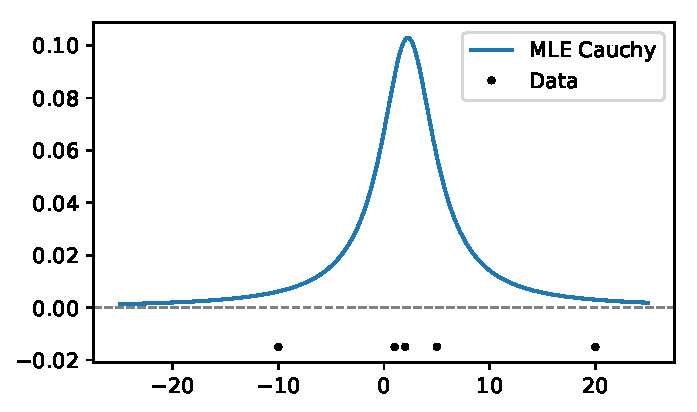
\includegraphics[width=0.5\textwidth]{./figs/Cauchy_MLE.pdf}
		\end{figure}
\end{itemize}

\newpage
\subsection{Exact inference examples}

\no Binomial model
\begin{itemize}
	\item Data: $D = \{(k_1, n_1), (k_2, n_2), \ldots, (k_N, n_N)\}$, where $k_i$ (successes), $n_i$ (attempts) $\in \mathds{N} \text{ and } k_i \leq n_i$
	\item Parameter: $p$ (probability of success) $\in [0,1]$, flat prior: $P(p) = 1$, on $[0,1]$
	\item Likelihood: $P(k_i \;|\; n_i, p) = \text{Binomial} (k_i\;|\;n_i, p) = {n_i \choose k_i} \; p^{k_i} (1-p)^{n_i - k_i}$
	\item Posterior: 
	\ba 
		P(p\;|\;D)
		&=& \frac{1}{Z} \prod_{i=1}^N \left[p^{k_i} (1-p)^{n_i - k_i}\right] = \frac{1}{Z} p^{k_\text{tot}} (1 - p)^{n_\text{tot} - k_\text{tot}} 
		\\
		&=& \frac{\Gamma(\alpha + \beta)}{\Gamma(\alpha)\Gamma(\beta)} p^{\alpha-1} (1-p)^{\beta-1} = \text{Beta}(p\;|\;\alpha = k_\text{tot} + 1,\beta = n_\text{tot} - k_\text{tot} +1),
	\ea
	where $k_\text{tot} = \sum_i k_i$ and $n_\text{tot} = \sum_i n_i$. Mean, mode and standard deviation are
	\ba
		&& \mathbb{E}(p) = \frac{\alpha}{\alpha + \beta} = \frac{k_\text{tot} + 1}{n_\text{tot} + 2}, 
		\quad 
		\text{mode}(p) = \frac{\alpha - 1}{\alpha + \beta -2} = \frac{k_\text{tot}}{n_\text{tot}},
		\\ 
		&& \text{std}(p) = \frac{\sqrt{\alpha \beta}}{(\alpha + \beta) \sqrt{\alpha + \beta + 1}} = \frac{\sqrt{(k_\text{tot} + 1)(n_\text{tot} - k_\text{tot} + 1)}}{(n_\text{tot} + 2)\sqrt{n_\text{tot} + 3}}
	\ea
\end{itemize}

\no Poisson model
\begin{itemize}
	\item Data: $D = \{k_1, k_2, \ldots k_N\}$, where $k_i$ (number of events) $\in \mathds{N}$
	\item Parameters: $\lambda$ (expected number of events) $ > 0$, flat prior: $P(\lambda) = \text{const.}$
	\item Likelihood: $P(k_i\;|\;\lambda) = \text{Poisson}(k\;|\;\lambda) = e^{-\lambda} \frac{\lambda^{k_i}}{k_i!}$
	\item Posterior: 
	\ba
		P(\lambda\;|\;D) 
		&=& \frac{1}{Z} \prod_{i=1}^N\left[e^{-\lambda} \lambda^{k_i}\right] = \frac{1}{Z} e^{-N\lambda} \lambda^{k_\text{tot}}
		= \frac{\beta^\alpha}{\Gamma(\alpha)} \lambda^{\alpha -1} e^{-\beta\lambda} = \text{Gamma}(\lambda\;|\; \alpha = k_\text{tot} + 1, \beta = N),
	\ea
	where $k_\text{tot} = \sum_i k_i$. Mean, mode and standard deviation are
	\ba
		\mathbb{E}(\lambda) = \frac{\alpha}{\beta} = \frac{k_\text{tot} + 1}{N},\quad \text{mode}(\lambda) = \frac{\alpha - 1}{\beta} = \frac{k_\text{tot}}{N},\quad
		\text{std}(\lambda) = \frac{\sqrt{\alpha}}{\beta} = \frac{\sqrt{k_\text{tot} + 1}}{N}
	\ea
\end{itemize}

\newpage
\no Multinomial model
\begin{itemize}
	\item Data: $D = \{(k_{1,1}, k_{1,2}, \ldots k_{1,M}), (k_{2,1}, k_{2,2}, \ldots k_{2, M}), \ldots (k_{N,1}, k_{N,2}, \ldots k_{N, M})\}$, where $k_{i,j}$ (counts of outcome $j$) $\in \mathds{N}$, and $\sum_{j}k_{i,j} = 1, \; \forall i$.
	\item Parameters: $p = (p_1, p_2, \ldots p_M)$, where $p_j$ (probability of outcome $j$) $ > 0$ and $\sum_j p_j = 1$; flat prior: $P(p) = \text{const.}$
	\item Likelihood: $P(\{k_{i,j}\}_{j=1}^M\;|\;p) = \text{Multinomial}(\{k_{i,j}\}_{j=1}^M\;|\;p) = k_{i,\text{tot}}! \prod_j \frac{p_j^{k_{i,j}}}{k_{i,j}!}$
	\item Posterior:
	\ba
		P(p\;|\;D) &=& \frac{1}{Z} \prod_{i=1}^N \prod_{j=1}^M (p_j)^{k_{i,j}} = \frac{1}{Z} \prod_{j=1}^{M} (p_j)^{k_{\text{tot}, j}} = \Gamma(\alpha_\text{tot}) \prod_{j=1}^M \frac{(p_j)^{\alpha_j - 1}}{\Gamma(\alpha_j)} = \text{Dirichlet}(p\;|\;\alpha_j = k_{\text{tot}, j} + 1),
	\ea
	where $k_{i,\text{tot}} = \sum_j k_{i,j}$, $k_{\text{tot}, j} = \sum_i k_{i,j}$, and $\alpha_\text{tot} = \sum_j \alpha_j = k_\text{tot,tot} + M$. Mean, mode and marginal standard deviation are
	\ba
		&& \mathbb{E}(p_j) = \frac{\alpha_j}{\alpha_\text{tot}} = \frac{k_{\text{tot},j} + 1}{k_\text{tot,tot} + M},
		\quad
		\text{mode}(p):\; p_j = \frac{\alpha_j-1}{\alpha_\text{tot}-M} = \frac{k_{\text{tot},j}}{k_\text{tot,tot}}
		\\
		&& \text{std}(p_j) = \frac{\sqrt{\alpha_j(\alpha_\text{tot} - \alpha_j)}}{\alpha_\text{tot}\sqrt{\alpha_\text{tot} + 1}} = \frac{\sqrt{(k_{\text{tot},j} + 1) (k_{\text{tot,tot}} - k_{\text{tot},j} + M - 1)}} {(k_{\text{tot,tot}} + M) \sqrt{k_{\text{tot,tot}} + M + 1}}
	\ea
\end{itemize}

\no Exponential model
\begin{itemize}
	\item Data: $D = \{t_1, t_2, \ldots t_N\}$, where $t_i$ (waiting times) $> 0$
	\item Parameter: $\gamma$ (rate) $> 0$, flat prior: $P(\gamma) = \text{const.}$
	\item Likelihood: $P(t_i\;|\;\gamma) = \text{Exponential}(t_i\;|\;\gamma) = \gamma e^{-\gamma t_i}$
	\item Posterior:
	\ba
		P(\gamma\;|\;D) &=& \frac{1}{Z} \prod_{i=1}^N \left[\gamma e^{-\gamma t_i}\right] = \frac{1}{Z} \gamma^N e^{-\gamma t_\text{tot}} = \frac{\beta^\alpha}{\Gamma(\alpha)} \gamma^{\alpha-1} e^{-\beta\gamma} = \text{Gamma}(\gamma\;|\;\alpha = N+1, \beta = t_\text{tot}),
	\ea
	where $t_\text{tot} = \sum_i t_i$. Mean, mode, standard deviation are
	\be
		\mathbb{E}(\gamma) = \frac{\alpha}{\beta} = \frac{N+1}{t_\text{tot}},\quad \text{mode}(\gamma) = \frac{\alpha -1}{\beta} = \frac{N}{t_\text{tot}}, \quad\text{std}(\gamma) = \frac{\sqrt{\alpha}}{\beta} = \frac{\sqrt{N+1}}{t_\text{tot}}
	\ee
\end{itemize}

\newpage
\no Normal
\begin{itemize}
	\item Data: $D = \{x_1, x_2, \ldots x_N\}$, where $x$ (value) $ \in \mathds{R}$
	\item Parameters: $\mu$ (expected value) $\in \mathds{R}$, $\sigma^2$ (variance) $ >0$, uninformative prior: $P(\mu, \sigma^2) = \text{const.}$
	\item Likelihood: $P(x_i\;|\;\mu, \sigma^2) = \text{Normal}(x_i\;|\;\mu, \sigma^2) = \frac{1}{\sqrt{2\pi \sigma^2}} \exp\!\left[-\frac{(x_i - \mu)^2}{2\sigma^2}\right]$
	\item Posterior:
	\ba
		P(\mu, \sigma^2\;|\;D) 
		&=& \frac{1}{Z}\prod_{i=1}^N \left\{\frac{1}{\sqrt{\sigma^2}} \exp\!\left[-\frac{(x_i-\mu)^2}{2\sigma^2}\right]\right\} = \frac{1}{Z} \left(\frac{1}{\sigma^2}\right)^{N/2} \exp\!\left[-\frac{Ns^2 + N(\mu - m)^2}{2\sigma^2}\right]
		\\
		&=&
		\frac{\sqrt{\lambda}}{\sqrt{2\pi \sigma^2}}\frac{\beta^\alpha}{\Gamma(\alpha)} \left(\frac{1}{\sigma^2}\right)^{\alpha + 1} \exp\!\left[-\frac{2\beta + \lambda(\mu - \mu_c)^2}{2\sigma^2}\right]
		\\
		&=& \text{Normal-Inverse-Gamma}\Big(\mu, \sigma^2\;\Big|\; \alpha = \frac{N-3}{2},\; \beta = \frac{Ns^2}{2},\; \mu_c = m,\; \lambda=N\Big),
	\ea
	where $m = \frac{1}{N}\sum_i x_i$ is the empirical mean, $s^2 = \frac{1}{N}\sum_i (x_i - m)^2$ is the empirical variance. 
	The mode is identical to the MLE result
	\be
		\text{mode}(\mu, \sigma^2) = (m, s^2).
	\ee
	The marginal, and mean, mode and standard deviation of $\mu$ is
	\ba
		P(\mu\;|\;D) 
		&=& \sum_{\sigma^2} P(\mu, \sigma^2\;|\;D) = \frac{\Gamma\left(\frac{N-2}{2}\right)}{\Gamma\left(\frac{N-3}{2}\right)} \frac{1}{\sqrt{\pi s^2}}\left[1 + \frac{(\mu - m)^2}{s^2}\right]^{-(N-2)/2}
		\\
		&=& \frac{\Gamma\left(\frac{\nu + 1}{2}\right)}{\Gamma\left(\frac{\nu}{2}\right)} \frac{1}{\sqrt{\pi \nu}}\left[1 + \frac{1}{\nu}\left(\frac{\mu - \text{loc}}{\text{scale}}\right)^2\right]^{-(\nu+1)/2} \frac{1}{\text{scale}} 
		\\ 
		&=& \text{t-distr}\Big(\mu\;\Big|\;\text{loc}=m,\; \text{scale}=\frac{s}{\sqrt{N-3}},\; \nu=N-3\Big),
	\ea
	\be
		\mathbb{E}(\mu) = m,\quad \text{mode}(\mu) = m,\quad \text{std}(\mu) = \frac{s}{\sqrt{N-3}} \sqrt{\frac{\nu}{\nu-2}} = \frac{s}{\sqrt{N-5}},
	\ee
	where $\nu$ is the ``degrees of freedom'' of the Student's t-distribution. The marginal, and mean, mode and standard deviation of $\sigma^2$ is
	\ba
		P(\sigma^2\;|\;D) &=& \sum_\mu P(\mu, \sigma^2\;|\;D) = \frac{\beta^\alpha}{\Gamma(\alpha)}\left(\frac{1}{\sigma^2}\right)^{\alpha+1} \exp\left(-\frac{\beta}{\sigma^2}\right)
		\\
		&=& \text{Inverse-Gamma}\Big(\sigma^2\;\Big|\;\alpha = \frac{N-3}{2},\;\beta = \frac{Ns^2}{2}\Big)
	\ea
	\be
		\mathbb{E}(\sigma^2) = \frac{\beta}{\alpha - 1} = s^2 \frac{N}{N-5},\quad \text{mode}(\sigma^2) = \frac{\beta}{\alpha + 1} = s^2\frac{N}{N-1}, \quad \text{std}(\sigma^2) = \frac{\beta}{(\alpha-1)\sqrt{\alpha-2}} = s^2\frac{\sqrt{2} N}{(N-5)\sqrt{N-7}}
	\ee
\end{itemize}

\newpage
\begin{figure}[h]
	\centering
	\includegraphics[width=\textwidth]{./figs/Exact-Inference-summary.pdf}
\end{figure}
